\chapter{Concept}
\label{sec:concept}

 % SELECTION APPLICATION, QUADTREE, USERSTUDY, VERGLEICHS-MAß

The goal of this work was to describe and implement a framework that allows for meaningful statements about differences between user selected regions of importance and computer generated mesh saliency maps to be made. It also included such a comparison on a basic, conceptual level. Based on these abstract tasks given, the workload and how I approached it, can be described by the following milestone-like, high level requirements.

\begin{enumerate}
	\item implement a selection application for the V2C's projection installation
	\begin{enumerate}
		\item spatial indexing of 3D data
		\item selection process
	\end{enumerate}
	\item conduct a user study to acquire data for a comparison
	\item conceptualise a measure of differences between the data sets
\end{enumerate}

In this section, I will go through these requirements and describe in more detail what specific challenges they entailed and how I went about implementing solutions to them. I will also describe the underlaying concepts I chose to use and how I amended them to better fit this work where needed.

	\section {Implementing a selection application for the V2C's projection installation}
	\label{sec:implementing_selection_application_v2c}
	% LRT = leibinz supercomputing centre(?)
One of the main challenges of this work was developing a piece of C++ software that allows users in the five-sided projection installation of the Leibniz Supercomputing Centre to select vertices of 3D objects using the existing soft- and hardware components at hand there. Designing, implementing and adjusting this software to being executable as a multi-threaded client-server application in said projection installation, was a challenging and time-consuming aspect of this work. For the rest of this work, this piece of software will be refferend to as \textit{selection application}. For details on its implementation, see section \ref{sec:selection_application}.

		\subsection{Spatial indexing of 3D data}
		\label{sec:impl_spatial_indexing_3d}
3D objects and data in general are read as lists of coordinates by computers. Common 3D file formats such as .OBJ, .FBX and .STL contain the same data in similar structures, using multiple lists of different kinds of geometric information. While they these formats vary in the range of information they can hold, they all represent at least the following types of essential data. \textit{Vertices}, or a three tuple of float values describing x, y and zu coordinates and \textit{faces}, or basic triangles consisting of three vertices. Other optinal information that can be represented include vertex normals, texture coordinates and more complex features such as assigned materials, animations and armature objects. Figure \ref{fig:obj_content} shows an excerpt of a 3D file in .OBJ format, viewed in a simple text editor (gedit).

\begin{figure}[htb]
  \centering
  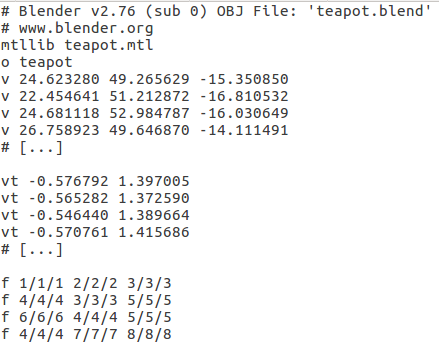
\includegraphics[width=.6\textwidth]{obj_content.png}\\ % PNG-File
  \caption{Notation in .OBJ format}\label{fig:obj_content}
\end{figure}

All these types of information share the following properties which were of relevance for this work. They are contiguous lists of lines, each line representing one instance of the data type indicated in the beginning of the line. Figure \ref{fig:obj_content} depicts an excerpt of an .OBJ file ocntaining vertices (lines starting with v), vertex texture coordinates (lines starting wit vt) and faces (lines starting with f).

These lists are not ordered. Depending on the modelling process, the vertices, faces and all the other attributes can be presented in an completely arbitrary order which hold very little information about the actual, geometric features of the object. The spatial position of any given vertex in relation to the entire object can not be retrieved from this type of notation. This created the demand for spatially indexing of 3D data in the scope this work.

I decided to implement the concept of Octrees \cite{Octree} because of its convenient characteristics as well as prior, personal working experience with \textit{quadtrees}. In an octree, the geometric size of the smallest possible leaf node can be determined in direct relation to the object to be indexed and, at any level, all leafs and nodes will be of the same size. This is highly useful in radius-based proximity-requests for multipl reasons as described in section \ref{sec:addVerticesToSelectionByCoordinates()}.

\begin{figure}[htb]
  \centering
  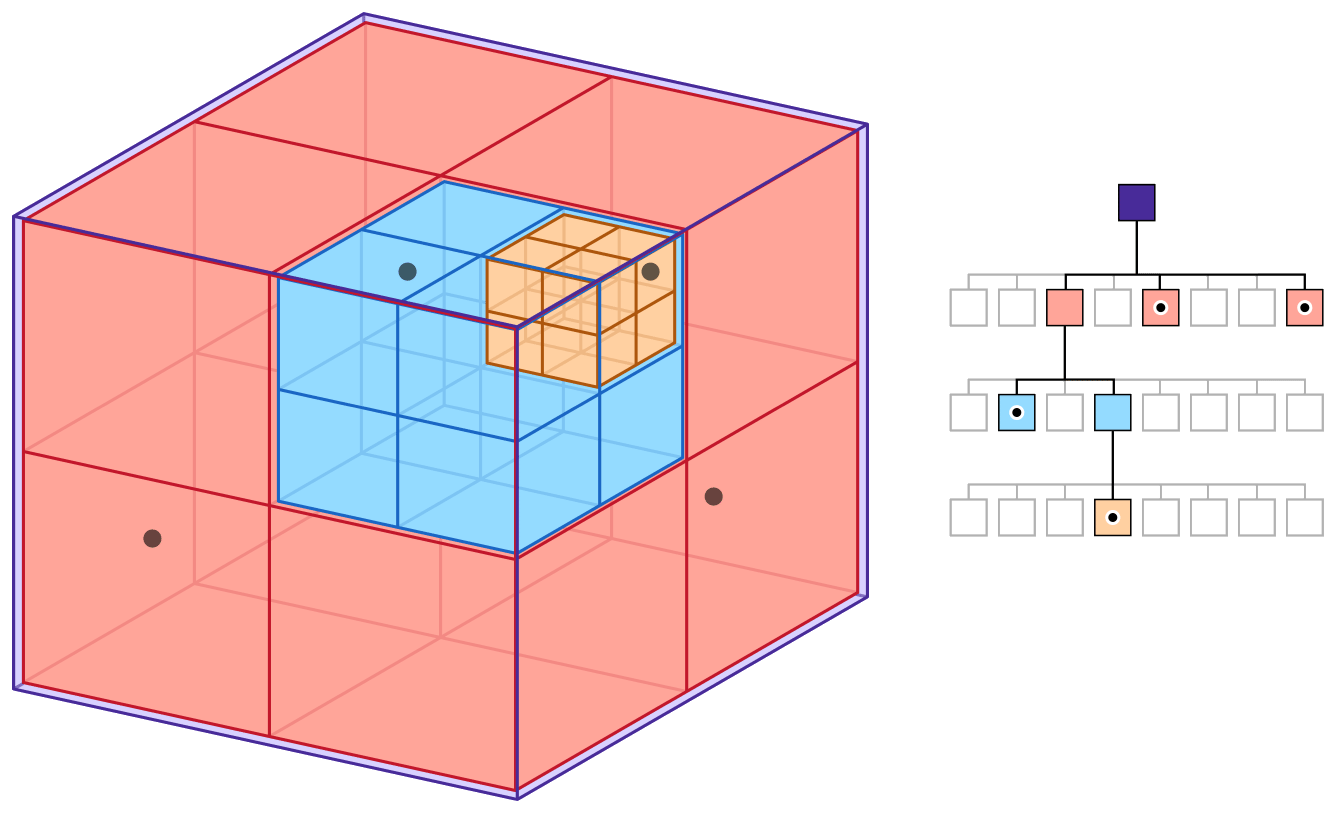
\includegraphics[width=.9\textwidth]{ocTree_apple.png}\\ % PNG-File
  \caption{An octree structure indexing four vertices. Left: 3D view, right: tree structure; 2017, https://developer.apple.com/documentation/}\label{fig:ocTree_apple}
\end{figure}

One of the most common queries performed on 3D data are proximity queries. This means that vertices located within a given radius around an input query-coordinate are to be retrieved. The trivial and obviously highly inefficient solution to such a problem would be to iterate through the entire list of vertices and their coordinates and check for those who fulfill this query condition. This is where spatial indexing structures such ad octree come into play. The concept of octrees is highly recursive and can realize all the most common types of queries (including search queries) in logarithmic time.

An octree is a set of nodes that store references to one another. The highest-level node is called the root node, bottom level nodes are usually referred to as leaf nodes or leafs. Every node that is not a leaf node has eight children-nodes which, in a spatial sense, make up the entire space of their parent node. Such non-leaf nodes can also be described as roots of subtrees.

Figure \ref{fig:ocTree_apple} taken from \cite{octAp} shows a simple octree structure indexing four vertices, both in 3D and tree view. Note how the root node on level 0, shaded purple on the right, is represented as a large purple cube on the left, encompassing the entire set of vertices. The figure clearly visualizes how an non-balanced octree structure that allows one vertex per leaf node at most would look like. On levels 1, 2 and 3, there are eight nodes each. On level 1, there are two leaf nodes that hold one vertex each, on level 2 and 3, there is one leaf holding one vertex.

The most important parameter for an octree is the maximum allowed number of vertices per leaf node. Once the dimensions in x-,y - and z-direction of the 3D object to be indexed have been determined, the root node of the octree will store every vertex until said maximum allowed number of vertices is reached. Up until that point, the root node was still a leaf. It is now a root no longer and will create eight new nodes (its child nodes) and store references to them. This process is repeated recursively for every new node until every leaf node holds less than the maximum allowed number of vertices per leaf node. It is worth mentioning that in many implementations of the octree concept, every leaf node needs to be at the same level. For this work, I decided to implement the non-balanced version of an octree where this is not the case. The reason for this is that in 3D objects, the data is not evenly distributed inside the entire space defined by its bounding box that. The vertices make up the surface of the model, inside and outside of it, there is no spatial information to be indexed at all.

		\subsection{Selection process}
		\label{sec:selection_process}

To gather data to compare with computer generated mesh saliency maps, tracking user input was needed. In the five-sided projection installation of the \cite{v2c}, 3D objects would be loaded and spatially indexed using octrees as described in the section above. Now, the selection function had to be implemented. Using a handheld input device, a so-called \textit{wand}, as depicted in figure \ref{fig:wand}, users can interact with the scene in two essential ways - navigation and performing arbitrary operations mapped to the device's buttons. Each such operation can, among other information, use the current position and rotation of the wand as parameters.

\begin{figure}[htb]
  \centering
  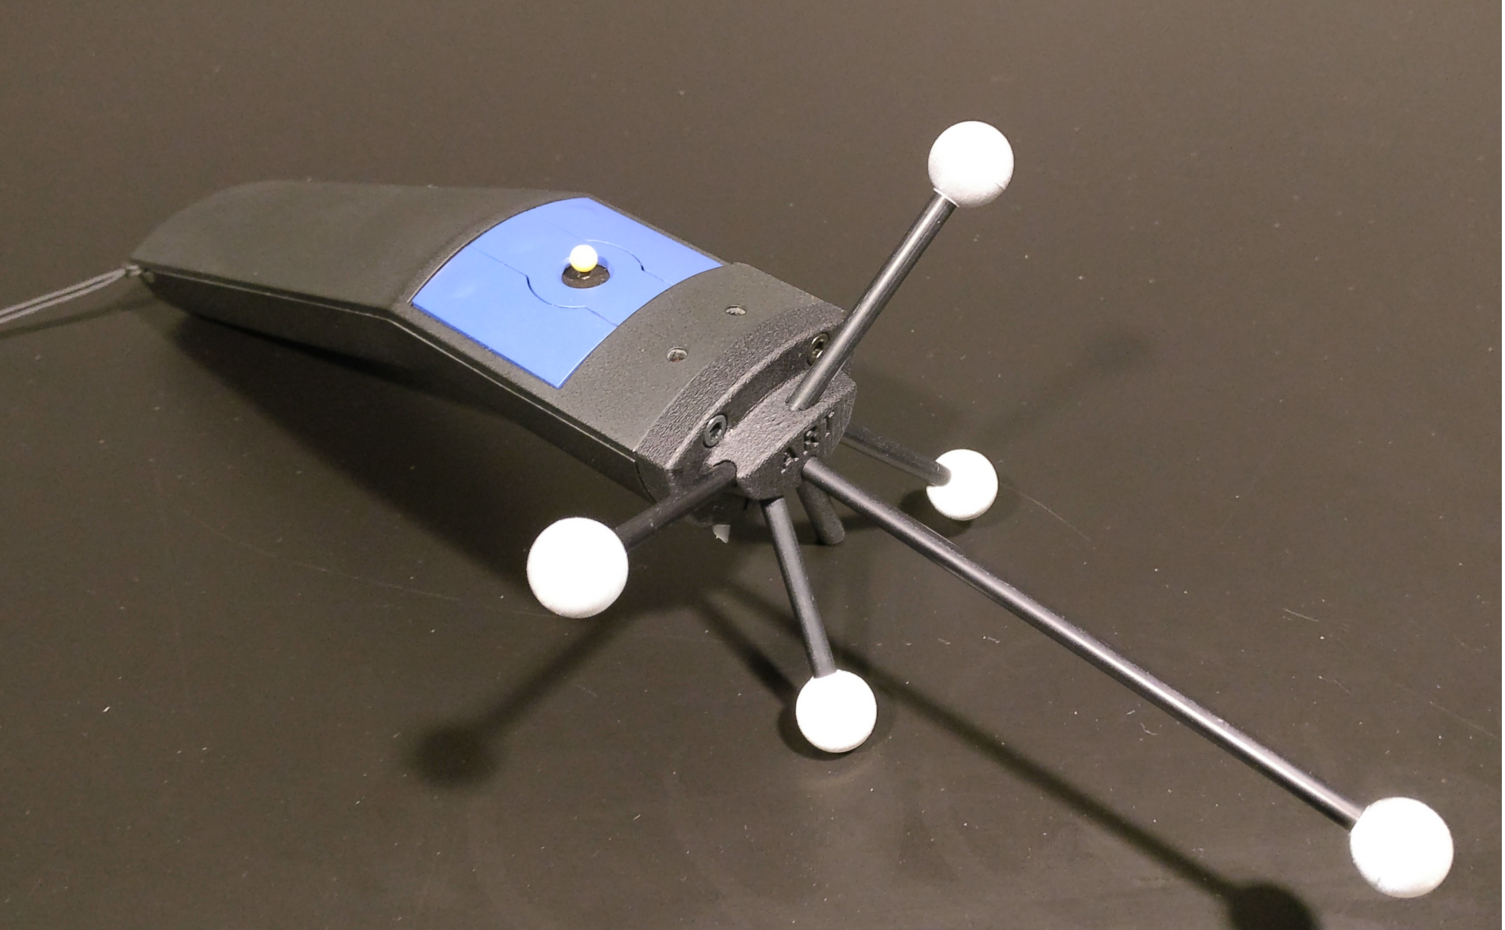
\includegraphics[width=.9\textwidth]{concept_wand.jpg}\\ % PNG-File
  \caption{The input device used at the V2C}\label{fig:wand}
\end{figure}

Figure \ref{fig:wand} depicts the \textit{wand} used in the V2C. The yellow joystick in the middle of its top side, in combination with the current rotation of the device, can be used to navigate the user's view onto the 
scene. The two essential functions of the application are mapped to two of the three buttons surrounding the joystick: The (from the perspective of a user holding the \textit{wand}) left button adds vertices near the current position of the wand to the vertex selection and the righthand button removes such vertices from it. The button in the middle does not have a function in this application, as well as the trigger-like fourth button on the button side of the \textit{wand} (not in view in the figure).
In accordance with the simplistic structure of the user study, the interaction was designed to be as little complex as possible, hence only these two buttons having actual, distinct purposes. 

With this setup in place, everything needed to implement the user selection part of the application is at hand. In order to provide as much visual accuracy as possible, a bright green diamond shaped object at the tracked position of the \textit{wand} is projected into the scene in addition to the loaded model. To additionally provide clear visual feedback, vertices selected are painted in bright red, clearly seperating them from non-selected parts of the object, displayed in plain grey. For more details on the visual presentation of the application, see 
% @TODO Verweis auf Kapitel User Study bzw. den Teil wo Fotos sind 1bauen

Whenever a user presses the left button of the \textit{wand}, a proximity query is performed on the octree structure indexing the object with its current position as the input. The position is passed as a \texttt{glm::vec3} variable, a basic 3D vector type provided by openGL's mathematics library. For a detailed description of how such a query is handled in this application, see section \ref{sec:addVerticesToSelectionByCoordinates()}.

In addition to these input coordinates, the following two parameters are passed to calls to this function in the context of a user adding or removing vertices to the current selection. The pre-computed selection radius as a \texttt{float} value and a reference to a temporary set of \texttt{size\_t} values called \texttt{intermediateSelection}, holding unique vertex IDs. After a query is terminated, the set of vertices found will be added to this temporary set.
Due to the design of the synchronisation routine between server and client threads of this application, this set will be emptied before the result of each such query is returend and written to it. If the \textit{add} button was pressed, the content of \texttt{intermediateSelection} will be added to another set holding the list of currently selected vertices total. If the \textit{remove} button was pressed, each of the temporarily selected vertices will be looked up in this second set and, in case it is found, removed from it. This approach prevents the total set of selected vertices to be sent from the server to all client threads at every frame during runtime. Only newly selected vertices (or those that are to be removed from the current selection) are sent across the application. The time for each action (in seconds since the application was started) is logged as well. 

	\section {Conduct user study with the selection application}
	\label{sec:conduct_user_study_with_the_selection_application}
% generell beschreiben (Aufbau, Ziel, Zusammenhang mit vorigen Sections), Details in eigenem grossen Kapitel
Another essential part of this work was conducting a user study where all of the aspects described in this chapter so far would be put to use. The goal was to collect data on what parts of 3D objects users found visually interesting or important. Users put on the stereoscopic, trackable glasses depicted in figure \ref{fig:glasses}, stepped inside the five-sided projection installation of the \cite{v2c} and were asked to mark regions of the object currently displayed that they considered to be intersting or important. The exact wording of the task given to participants in the user study reads as follows.

\textit{Please select parts and regions of the object that}

\begin{itemize}
	\item \textit{you would consider visually interesting or important}
	\item \textit{you would assume are natural focus points of attention}
	\item \textit{are vital for identifying the object}
\end{itemize}

After taking up to five minutes getting familiar with navigating and interaction within the projection installation, as well as selecting and deselecting vertices with the wand (\ref{fig:wand}, the main part of the user study began. 

\begin{figure}[htb]
  \centering
  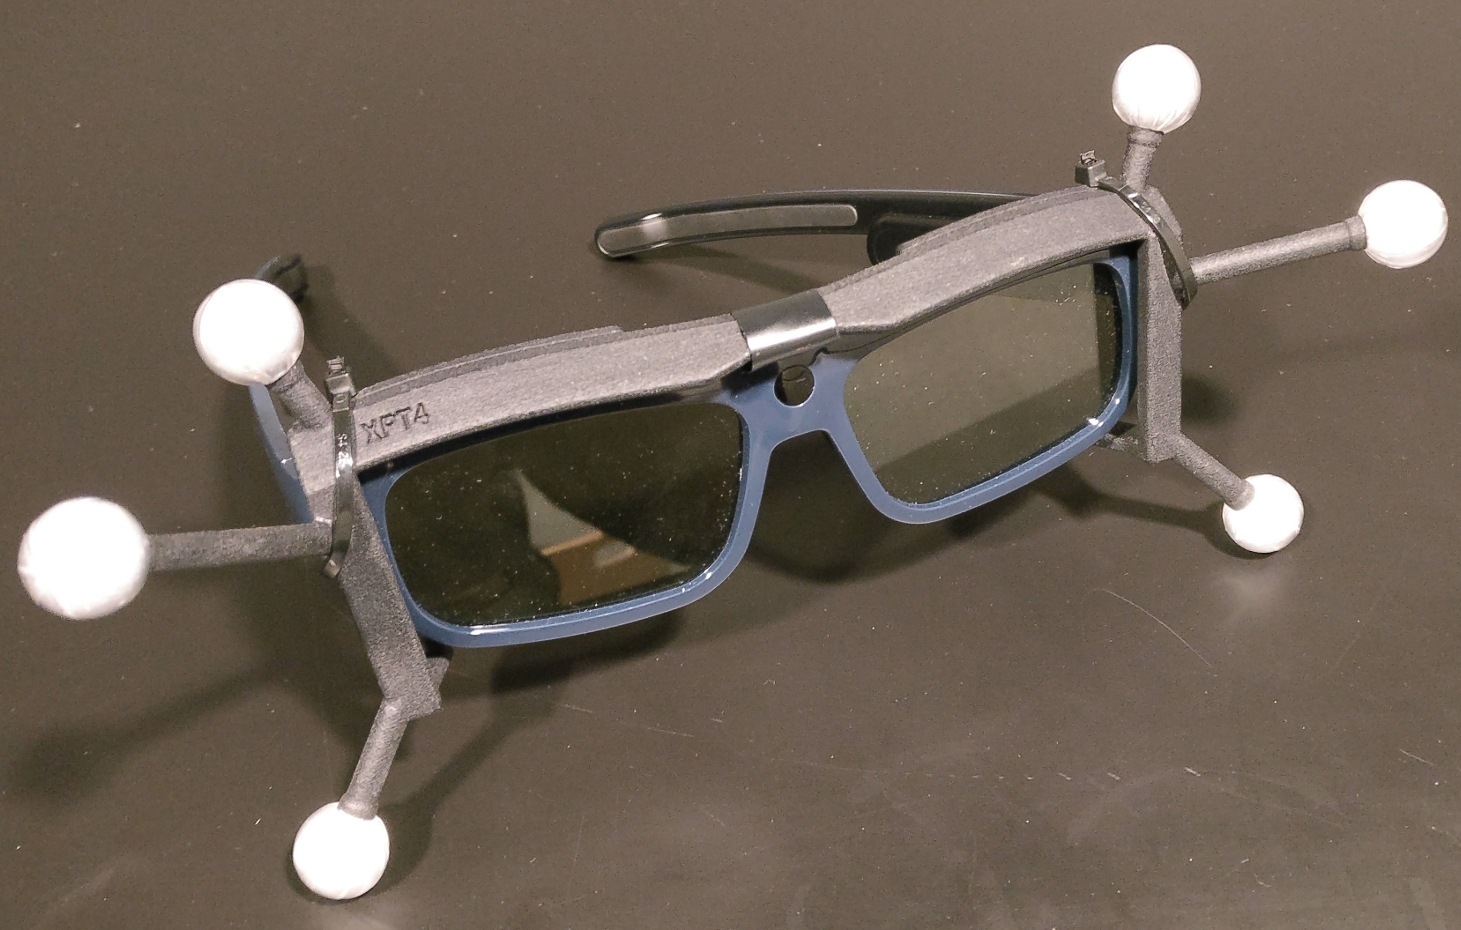
\includegraphics[width=.9\textwidth]{concept_glasses.jpg}\\ % PNG-File
  \caption{The trackable, stereoscopic glasses used at the V2C}\label{fig:glasses}
\end{figure}

Selections of the users would be gathered to compute user-weighted importance maps for the displayed 3D objects. These would be compared to previously computed mesh saliency maps. For the results and discussion of this comparison, see chapter 
% @TODO ref zu chapter "results usw" 1fügen. Selbiges davor noch anlegen

In this selection application, selection and deselection operations are executed with the current tracked position of the \textit{wand} as input coordinates. To give users a clear, live feedback on that tracked position, for every frame, a ten-sided, diamond-shaped object was also rendered in the scene on that very position. The object is shaded in a bright green, to be easily distinguishable within the 3D scene. However, it did not offer a visual representation of the pre-computed selection radius. Again, this radius $r_{max}$ is defined as $d_{min}$ / $2^{l_{max}}$ * 0.95, in other words 95\% the size of the smallest possible leaf node, so it is slightly different for every object loaded in the application. I chose not to adapt the size of the ten-sided object representing the position of the wand and keep it the same size for every object with the intention of providing more consistency within the scene, independent of the currently loaded object. This was also a design decision that went in accordance with the minimalistic general visual presentation of the application, as described in the following brief summary.

\begin{itemize}
	\item background-color of the application: (almost) black
	\item shader used for the loaded object: light grey, no textures, normals used
	\item shader used for selected vertices: bright red
	\item shader used for diamond-shaped object indicating the tracked position of the \textit{wand}: bright green
\end{itemize}

% @TODO: Bild rausrendern (user mit Wand in der Hand, geladenem Object + wand_pos), schneiden und uploaden

Regarding objects used for the study, I aimed at offering as much variety of types of objects among as few objects as possible. The motivation for this was to achieve results that are genereally applicable for any type of geometric data, at least to an basic extent. Also, to avoid the users losing motivation due to repeating tasks during the study, keeping the number of objects to a minimum was another constraint to be considered.
I decided to use three objects described table in \ref{tab:userstudy_objects} and depicted in figure \ref{fig:all_objects}.

\begin{table}[]
\centering
	\begin{tabular}{l|l|l|l|l}
		object	& created through	& source	& vertex count	& class of objects	\\ \hline
		cow	& 3D modelling		& \cite{cow}	& 69,648	& purely natural	\\
		P51 Mustang	&	3D modelling	& \cite{P51}	& 51,708	& purely mechanical	\\
		bunny sculpture	&	3D scan	& \cite{bun}	& 68,754	& natural, man-made	
	\end{tabular}
	\caption{3D objects used in the study}
	\label{tab:userstudy_objects}
\end{table}
% table 3.1

\begin{figure}[htb]
  \centering
  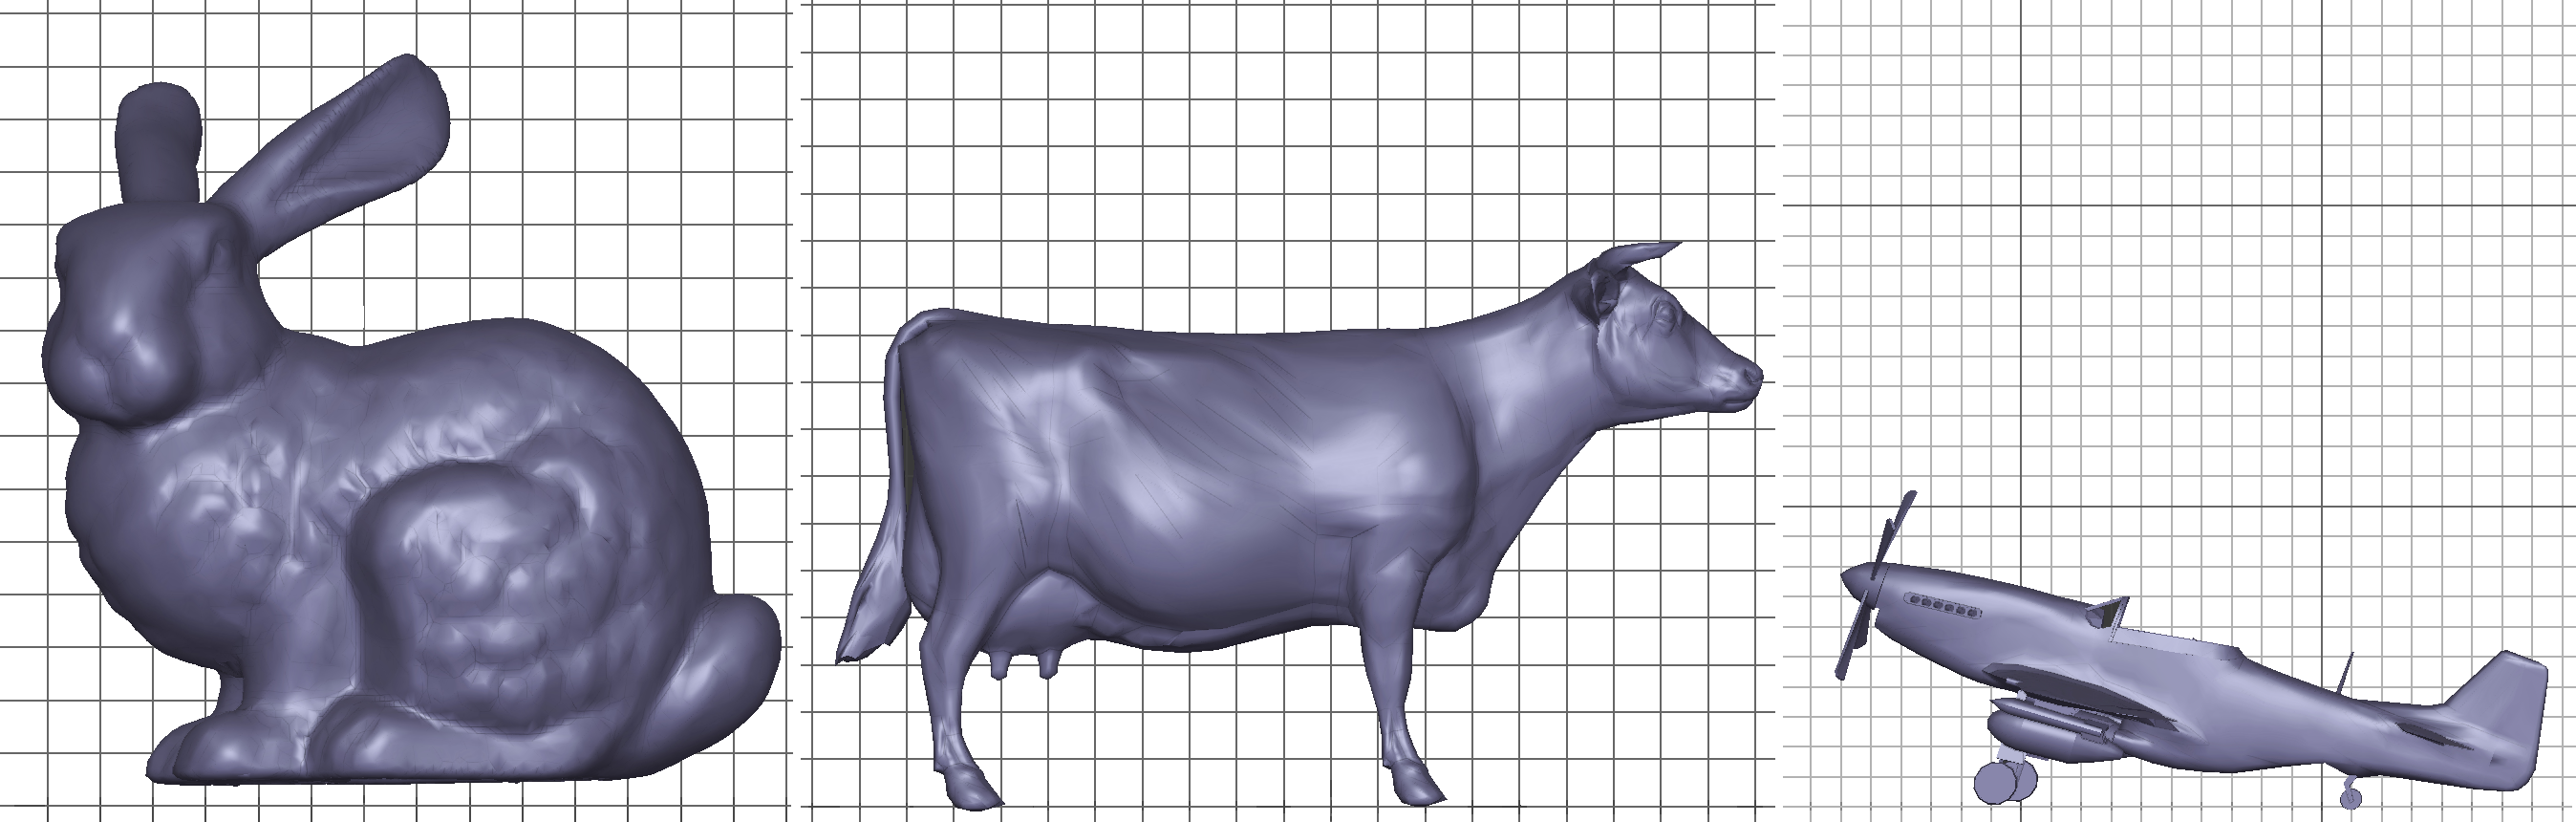
\includegraphics[width=1.0\textwidth]{userstudy_all_objects.png}\\ % PNG-File
  \caption{The 3D objects used for the user study}\label{fig:all_objects}
\end{figure}

Figure \ref{fig:all_objects} shows the objects used in the user study. From left to right, the 3D scanned bunny, the modelled cow and the low-poly, modelled aircraft are shown. Consider the grid to get a sense of their proportions. I did not scale them according to their real world sizes and instead made them take up approximately equal space in the virtual scene. This was done with the intention to provide a similar level of visual detail, independent of the actual geometric level of detail, for each object. %@TODO: Markus nach besserer Begründung fragen

I took two steps to eliminate the possibility of user selections being influenced by them first having to adapt to and getting familiar with the selection application. First, Every user was given five minutes to get familiar with the navigation and selection workflow. Selections made here were not considered for the results of the userstudy. After that, the three objects were presented in a randomly chosen order for five minutes each. The users were given the tasks stated at the beginning of this section and were free to use as much of the five minutes as they wanted to perform vertex selection and deselection operations.

The five minute time limit was an absolute upper limit for each selection process. Users were free to end selection prematurely whenever they stated they were satisfied with the selection as it is.

Besides the five minute \textit{tutorial phase} - the time users could take to get familiar with the application - and the actual tasks to be fulfilled (as described at the beginning of this section), only one more minor request was asked to be considered by users: An approximate symmetrical selection, meaning that, in cases where it was possible, parts of objects users selected on one side of an object would also be selected on the opposite side. Other than that, no additional information or hints were given. Users were told that there is no \textit{correct} way of to fulfill the selection task. They were encouraged to select whatever they deemed relevant according to the tasks based on their personal judgement.

	\section {Measure of differences}
	\label{sec:measure_of_difference}
Since a large portion of the workload of this work was the implementation of the selection application itself, as well as customizing it to the point it is executable in the V2C, the comparison of user generated and pre-computed mesh saliency maps was designed to be quick and easy. In this chapter I will describe how I conceptualised a basic way to compute a \textit{difference ratio}, normalised to a decimal value between 0 and 1, describing how much user saliency maps differ from mesh saliency maps. It is based on a simple vertex-wise comparison of saliency-values and makes use of the proximity queries provided by the octree structure, which is also the basis for the selection application itself as described in section \ref{sec:spatial_indexing_via_octree}.

In chapter % @TODO ref zu chapter "results usw" 1fügen. Selbiges davor noch anlegen
I consider both \textit{raw} and \textit{weighted difference} values, for a detailed explanation of these terms, see the following subsections. For a brief summery and step-wise explanation, see subsection \ref{sec:ste_wise_summery}.

		\subsection{Terms and abbreviations}
		\label{sec:concept_terms_and_abbreviations}
% @TODO threshold einbauen!! Hier und im Quelltext
The following terms, symbols and abbreviations will be used in the subsequent sections to explain the measure of difference used in this work.

\begin{description}
	\item [user saliency map] - a saliency map for an object based on the average times each vertex was selected by users
	\item [mesh saliency map] - a saliency map for an object that was computed as described in \cite{lee2005mesh}
	\item[difference ratio] - a float number, normalised to a value between 0.0 and 1.0 indicating how much the generated \textit{user saliency map} differs from the pre-computed \textit{mesh saliency map}, based on unweighted (raw) difference values
	\item[weighted difference ratio] - a float number, normalised to a value between 0.0 and 1.0 indicating how much the generated \textit{user saliency map} differs from the pre-computed \textit{mesh saliency map}, based on weighted difference values
	\item[$N(vi)$] - a part of an object consisting of multiple vertices $v_1$, ... $v_j$ which are located in a certain radius $r$ around currently considered vertex $v_i$
	\item[$v_i$] - the currently considered vertex \textit{i} $\in$ set of all vertices $V$ belonging to an object
	\item[$S_{M}(v_i)$] - the computed mesh saliency value for $v_i$
	\item[$S_{U}(v_i)$] - the user generated saliency value for $v_i$
	\item[$\Delta_{raw}(v_i)$] - the unweighted (raw) difference between the user and mesh saliency values $S_{U}(v_i)$ - $S_{M}(vi_i)$. The absolute value of the result is normalised to a value between 0.0 and 1.0
	\item[$\Delta_{weighted}(v_i)$] - the weighted difference between the user and mesh saliency values $S_{U}(v_i)$ - $S_{M}(vi_i)$. The absolute value of the result is normalised to a value between 0.0 and 1.0
	\item[$V_{proximty}(v_i)$] - a \textit{proximity set} of vertices $v_1$, ... $v_j$ that are located within radius $r$ around the coordinates of given vertex $v_i$
	\item[$\omega$] - a threshold value derived from mesh saliency values $S_{M}(v_1)$, ... $S_{M}(v_j)$ for all vertices $v_1$, ... $v_j$ $\in$ a \textit{proximity set} $V_{proximty}(v_i)$ of $vi$
\end{description}

		\subsection{unweighted difference ratio}
		\label{sec:unweighted_difference_ratio}
As stated above, $\Delta_{raw}(v_i)$, or the unweighted (raw) difference between user generated and computed mesh saliency value can easily be obtained by taking the absolute value of $S_{M}(v_i) - S_{U}(v_i)$. For each of the objects used in the user study, we computed a mesh saliency map using \texttt{climberpi's} implementation of \textit{mesh saliency} \cite{clms}, providing $S_{M}(v_i)$ for every vertex $v$ in $V_{bunny}$, $V_{cow}$ and $V_{P-51}$ where $V_{l}$ is the set of all vertices that make up the object with label $l$.

Values $S_{U}(v_i)$ are computed via a simple, average-based comparison of how many users selected each vertex. As mentioned in \ref{sec:user_selection}, user selections are written to simple structured text files containing one unique vertex ID and the time they were added to the selection (in seconds since the application was started) in every line, seperated by a tab symbol as depicted in table \ref{tab:user_selection_log_file}.

\begin{table}[]
\centering
	\begin{tabular}{l|l}
	vertId & timestamp \\ \hline
	27 & 64 \\
	59 & 62 \\
	63 & 62 \\
	64 & 62 \\
	65 & 62 \\
	67 & 62 \\
	68 & 62 \\
	69 & 62
	\end{tabular}
	\caption{Sample content of a user selection log file}
	\label{tab:user_selection_log_file}
\end{table}
% table 3.3

In the simple evaluation tool used for this work, before each logfile is read, a \texttt{std::vector<size\_t, int>} is created with size equivalent to the number of vertices of the currently considered object. After the last log file is processed, this \texttt{set} $userselections$ contains a mapping for each vertex $v_i$, describing how many users selected it with the \texttt{int} value at offset $i$, which equals the vertex ID represented as a \texttt{size\_t} value. In other words, let $userselections[i] = t$ for each vertex $v_i$ of an object where $t$ is the amount of users that selected $v_i$.

Next, the maximum number of times one or multiple vertices were selected $t_{max}$ is computed. Based on this maximum value, \textit{user saliency} values are $S_{U}(v_i)$ generated as follows.

$S_{U}(v_i) = userselections[i]/t_{max}$

\textit{User saliency} values for each of most selected vertices - those selected by $t_{max}$ users - will be 1.0, and 0.0 for those which were not selected by a single user. Every other \textit{user saliency} value will be somewhere in that range, describing what one could informally call the \textit{popularity} of the vertices.

With both \textit{mesh} and \textit{mesh saliency} values for each vertex $v_i$, we can use the absolute value of their difference as the \textit{unweighted (raw) difference}. The final step to generate the overall \textit{unweighted difference ratio} is a simple addition of $S_{U}(v_i)$ values for every $v_i \in V$, where $V$ is the total number of one object and dividing the result by $V$. This ratio gives a quick, first impression of how much the average user selection differs from a \textit{mesh saliency map} computed according to \cite{lee2005mesh}.

		\subsection{weighted difference ratio}
		\label{sec:weighted_difference_ratio}
The unweighted \textit{difference ratio}, being very basic and average based, lacks expressiveness. During research and preparation for this work, it became clear that \textit{mesh saliency maps} offer a solid basis for prediction models of what parts of 3D objects human attention tends to gravitate towards. By further developing and refining the concept, these predictions became precice and reliably, see chapter \cite{sec:related_work}. I based my idea for the \textit{weighted difference ratio} on the assumption that differences in saliency values for some vertices are more interesting than others.

\begin{figure}[htb]
  \centering
  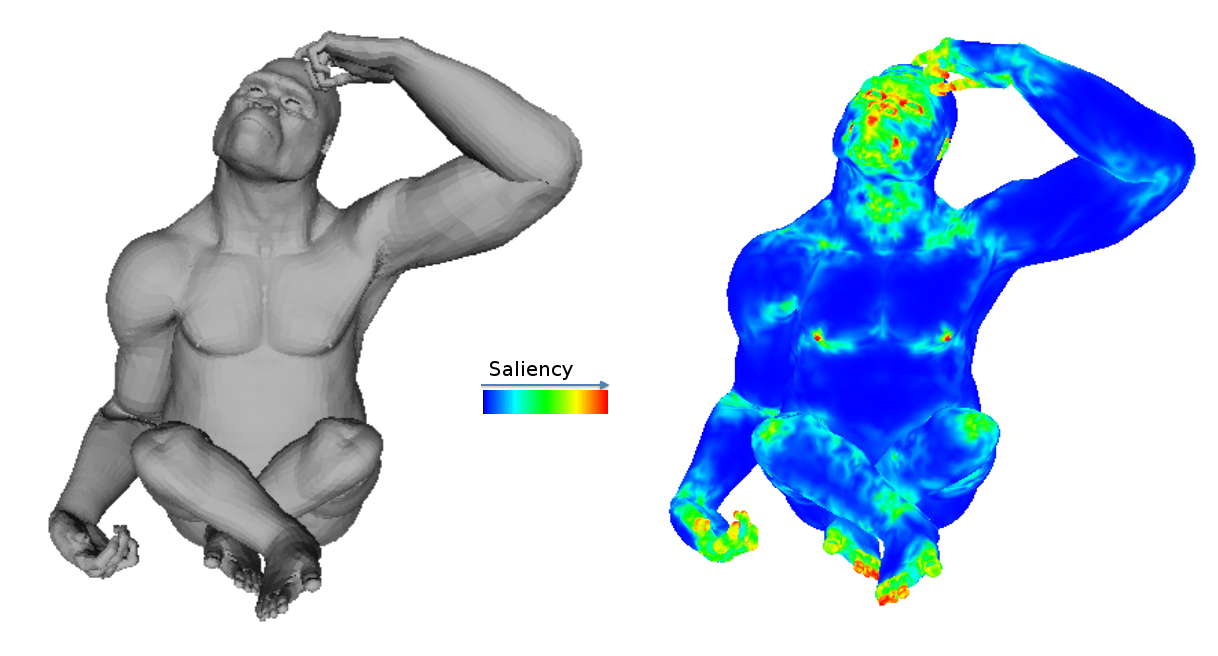
\includegraphics[width=1.0\textwidth]{mss_gorilla_alpha.png}\\ % PNG-File
  \caption{A multi-scale mesh saliency map for an object including color scale. Published by Nouri \textit{et al.} \cite{nouri2015multi}}\label{fig:gorilla_saliency_map}
\end{figure}

Consider figure \ref{gorilla_saliency_map}. It depicts an object and its multi-scale mesh saliency map as well as a scale for reference. The scale describes how yellow and red colored vertices indicate high mesh saliency values for those vertices while green and blue colored ones suggest lower values. Note that this map was not computed via the \textit{standard} mesh saliency model but an enhanced, multi-scale based one. The figure is suitable to explain the idea behind which point-wise difference value in user and mesh saliency values are \textit{weighted} in this work.

Based on the assumption that a very low \textit{user saliency value} of vertices which lays in a yellow or red shaded area is more interesting than one that is located in a green or blue area, I based the decision which vertex-wise difference ratios would be weighted on a comparison of other vertices surroundind them. Consider a vertex $v_i$ in the following cases.

\begin{description}
	\item [case 1:] $v_i$ has a \textit{user saliency} value of 0.2 or lower and vertices located in its proximity have an average \textit{mesh saliency} value of 0.8 or higher.
	\item [case 2:] $v_i$ has a \textit{user saliency} value of 0.2 or lower and vertices located in its proximity have an average \textit{mesh saliency} value of 0.3 or lower
	\item [case 3:] $v_i$ has a \textit{user saliency} value of 0.8 or higher and vertices located in its proximity have an average \textit{mesh saliency} value of 0.8 or higher
	\item [case 4:] $v_i$ has a \textit{user saliency} value of 0.8 or lower and vertices located in its proximity have an average \textit{mesh saliency} value of 0.3 or lower
\end{description}

I decided to base this simple evaluation process on the assumption that realistic, reliable results are achieved by the model of \textit{mesh saliency}. So I focused on finding deviations within parts and regions of objects that have higher mesh saliency values. Thus, only in cases 1 and 3, vertex-wise differences get weighted. High vertex-wise differences in regions that with a low overall mesh saliency value still are considered for the final \textit{weighted difference ratio}, but not as much as those that that emerge from cases 1 and 3.
% @TODO: 0.2? Hier beschreiben und im Quelltext ggf anpassen (threshold = average_saliency_val oder sowas)

Regarding how the actual weighting is done, a simple function that increases the vertex-wise \textit{raw difference} values, normalizes between 0.0 and 1.0 without getting greater than 1.0. So I chose to use an altered, restricted function describing a circle that has its centre at $x = 1.0, y = 0.0$ and radius $r = 1.0$. See figure{da unte halt}
% @TODO: Bild 1fuegen

\begin{figure}[htb]
  \centering
  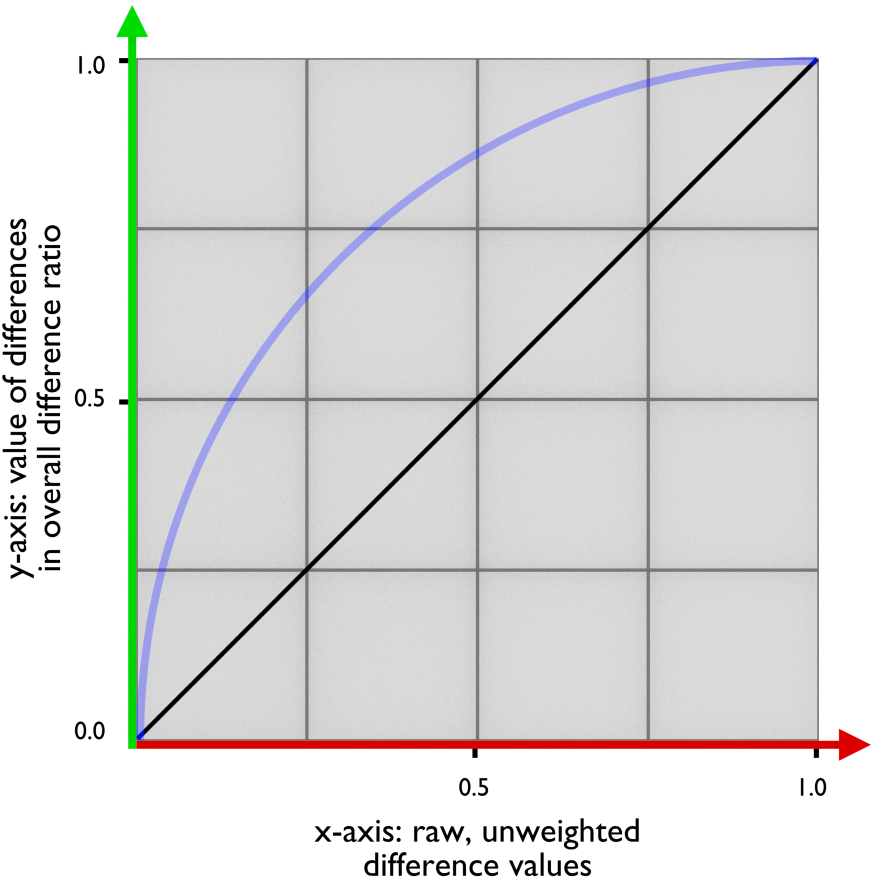
\includegraphics[width=.5\textwidth]{weighting_function.png}\\ % PNG-File
  \caption{Graphic representation of the weighting function in relation}\label{fig:weighting_function}
\end{figure}

		\subsection{step-wise summery}
		\label{sec:ste_wise_summery}
% @TODO: Comments (beginnend z. 678) aus Quelltext copy-pasteten
